\begin{abstract}
I am proposing two emojis for \textbf{NEURODIVERSITY}

\begin{figure}[h!]
\caption{Neurodiversity Emoji Concept Art}
\centering
  \subfloat[Emoji A: Rainbow Brain]{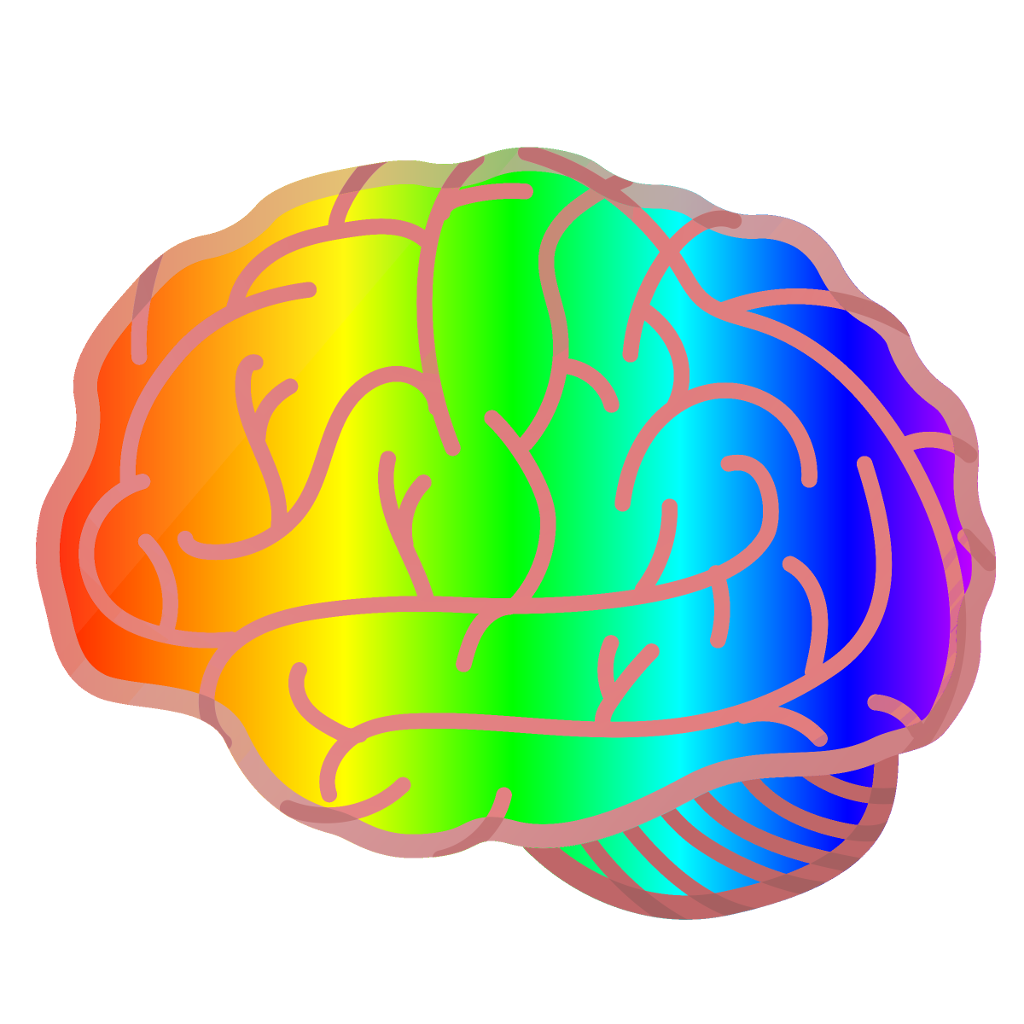
\includegraphics[width=0.333\textwidth]{neurodiversity.png}}
  \qquad
  \subfloat[Emoji B: Rainbow Infinity Loop]{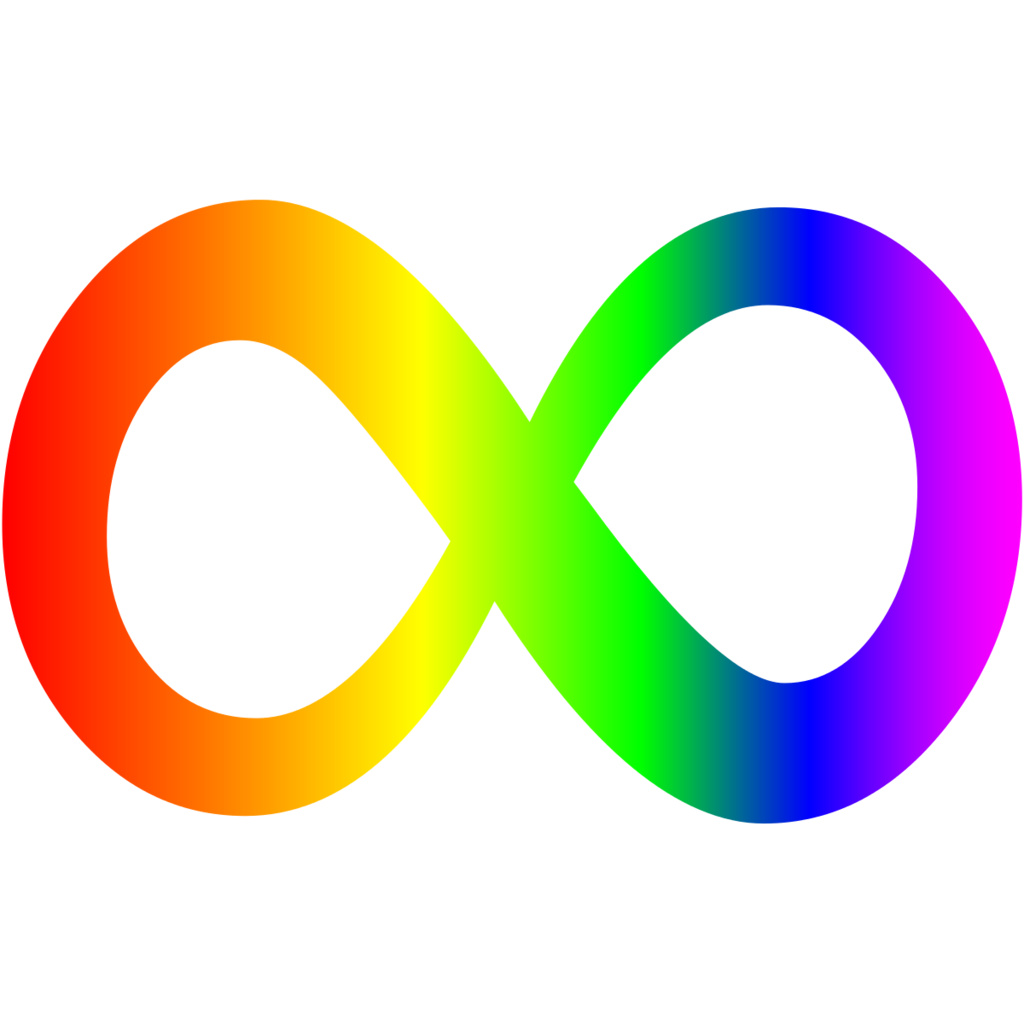
\includegraphics[width=0.333\textwidth]{SpectrumInfinity.png}}
%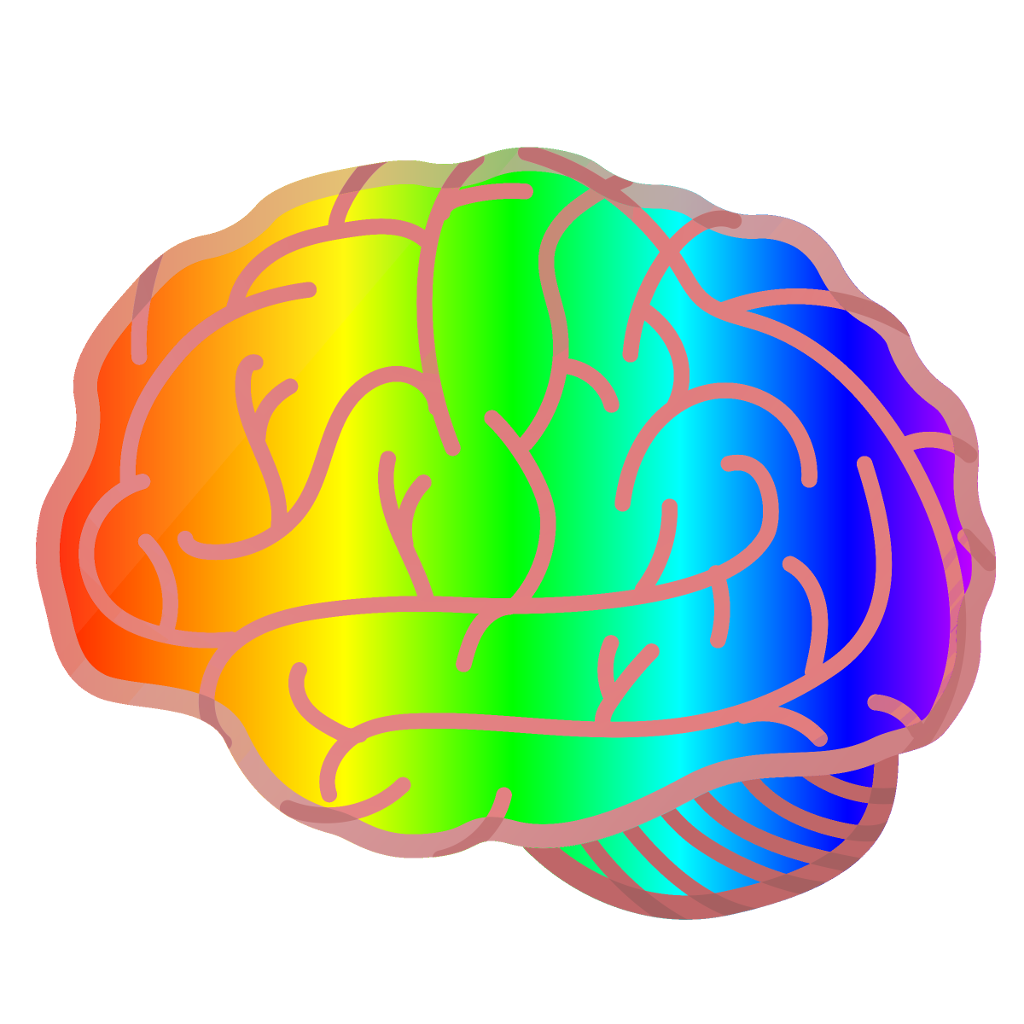
\includegraphics[width=0.333\textwidth]{neurodiversity.png}
\label{fig:neurodiversity}
\end{figure}

This is a very rough draft and is subject to radical change.

When used in a normal paragraph, the rainbow brain concept art renders as
$\vcenter{\hbox{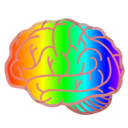
\includegraphics[height=\baselineskip]{neurodiversity128.png}}}$
and the rainbow infinity loop renders as
$\vcenter{\hbox{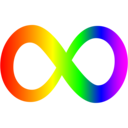
\includegraphics[height=\baselineskip]{SpectrumInfinity128.png}}}$
giving some idea of how they would render when compared to the similar
existing emojis \brainemoji{} and \infinityemoji{}.

Autism (often referred to as Autism Spectrum Disorder) refers to a spectrum of
characteristics that are the result of a neurologically
atypical brain. Typical characteristics include repetitive behaviors, differences in language
processing, difficulty in social interactions, and differences in how emotions and
empathy are expressed.

The center for disease control estimates that roughly 1 in 59 eight year olds is
autistic\footnote{\url{https://www.autism-society.org/news/2018-cdc-autism-incidence-rate-statement-from-the-autism-society/}}.
Generally biological boys \textit{(XY chromosome pair)} are more likely to be diagnosed as
autistic than biological girls \textit{(XX chromosome pair)}, though that
may be due to differences in social constructs regarding the expected behavior of
biological boys and biological girls resulting in a higher percentage of autistic
biological girls going undiagnosed.

As online social networking makes it easier for autistic individuals to find each
other, our positive identity as a demographic rather than a negative identity as a
disorder is starting to grow.

We believe emojis to express our neurodiverse identity, emojis chosen by our
community, are both warranted and will help us continue to identify each other and
grow as a community, enabling us to receive the important peer support we often
lack from society at large. Two are proposed because there are two different
pictographs currently in use by the community to represent neurodiversity that can
not be adequately represented by existing emojis.

The primary difference between those who are autistic and those who are not is in
how our brain works. A rainbow represents the full spectrum of visible light.

Some of us see a rainbow brain as a logical represention of the neurodiverse spectrum
that makes up our community. Others prefer a rainbow infinity loop.

Many members of the Neurodiverse community already identify with either the rainbow
brain or the rainbow infinity loop shown in figure~\ref{fig:neurodiversity}.

We respectfully request that one or preferably both be added to the official Emoji list.
\end{abstract}
